\chapter{Specifikacija programske potpore}
		
	\section{Funkcionalni zahtjevi}
			
			\noindent \textbf{Dionici:}
			
			\begin{packed_enum}
				
				\item Korisnici			
				\begin{packed_enum}
					
					\item Polaznik
					\item Predavač	
				\end{packed_enum}		
				\item Razvojni tim
				
			\end{packed_enum}
			
			\noindent \textbf{Aktori i njihovi funkcionalni zahtjevi:}
			
			
			\begin{packed_enum}
				\item  \underbar{Neregistrirani korisnik (inicijator) može:}
				
				\begin{packed_enum}
					
					\item registrirati se u sustav
					\begin{packed_enum}
						
						\item  stvoriti novi korisnički račun polaznika za koji su mu potrebni korisničko ime, lozinka, ime, prezime, e-mail adresa i broj kartice za naplatu \textbf{ili}
						\item  stvoriti novi korisnički račun predavača za koji su mu potrebni korisničko ime, lozinka, ime, prezime, e-mail adresa i IBAN računa, uz opciju stavljanja svoje slike i kratke biografije
				
					\end{packed_enum}
	
				\end{packed_enum}
			
				\item  \underbar{Predavač (inicijator) može:}
				
				\begin{packed_enum}
					
					\item pregledavati i mijenjati osobne podatke
					\item pretraživati ponuđene tečajeve
					\item dodati, urediti i obrisati tečaj
					\item pregledati polaznike svojih tečajeva
					\item prihvatiti ili odbiti termin konzultacija
					
				\end{packed_enum}
			
			\eject
			
				\item  \underbar{Polaznik (inicijator) može:}
				
				\begin{packed_enum}
					
					\item pregledavati i mijenjati osobne podatke
					\item pretraživati ponuđene tečajeve
					\item upisati i platiti tečaj
					\item pristupiti plaćenom tečaju
					\item preuzimati materijale upisanog tečaja
					\item poslati zahtjev za konzultacijama
					
				\end{packed_enum}
			
			
				\item  \underbar{Baza podataka (sudionik):}
				
				\begin{packed_enum}
					
					\item pohranjuje sve podatke o korisnicima
					\item pohranjuje sve podatke o tečajevima i njihove materijale
					
				\end{packed_enum}
			\end{packed_enum}
			
			\eject 
			
			
				
			\subsection{Obrasci uporabe}
				
				
				\subsubsection{Opis obrazaca uporabe}

					\noindent \underbar{\textbf{UC1 - Registracija}}
					\begin{packed_item}
	
						\item \textbf{Glavni sudionik:} Korisnik
						\item  \textbf{Cilj:} Izbor maila i korisničkog imena
						\item  \textbf{Sudionici:} Baza podataka
						\item  \textbf{Preduvjet:} -
						\item  \textbf{Opis osnovnog tijeka:}
						
						\item[] \begin{packed_enum}
	
							\item Korisnik unosi potrebne podatke
							\item Korisnik je usmjeren na stranicu za unos dodatnih podataka (\hyperref[UC2] {UC2})
							
						\end{packed_enum}
						
						\item  \textbf{Opis mogućih odstupanja:}
						
						\item[] \begin{packed_item}
	
							\item[1.a] Odabir već zauzetog korisničkog imena i/ili e-maila, unos korisničkog podatka u nedozvoljenom formatu ili pružanje neispravnog e-maila
							\item[] \begin{packed_enum}
								
								\item Sustav obavještava korisnika o neuspjelom upisu i vraća ga na stranicu za registraciju
								
							\end{packed_enum}
							
						\end{packed_item}
					\end{packed_item}
									
					\noindent \label{UC2} \underbar{\textbf{UC2 - Unos podataka}}
					\begin{packed_item}
						
						\item \textbf{Glavni sudionik:} Korisnik
						\item  \textbf{Cilj:} Stvoriti korisnički račun za pristup sustavu
						\item  \textbf{Sudionici:} Baza podataka
						\item  \textbf{Preduvjet:} Uspješan unos e-mail adrese i korisničkog imena
						\item  \textbf{Opis osnovnog tijeka:}
						
						\item[] \begin{packed_enum}
							
							\item Korisnik unosi potrebne podatke
							\item Korisnik prima obavijest o uspješnoj registraciji
							
						\end{packed_enum}
						
						\item  \textbf{Opis mogućih odstupanja:}
						
						\item[] \begin{packed_item}
							
							\item[1.a] Ostavljen prazan jedan od potrebnih podataka
							\item[] \begin{packed_enum}
								
								\item Sustav obavještava korisnika da mora unijeti podatak
								
							\end{packed_enum}
							\item[1.b] Korisnik odustaje od registracije
							\item[] \begin{packed_enum}
								
								\item Sustav briše cijelu registraciju
								
							\end{packed_enum}
							
						\end{packed_item}
					\end{packed_item}
			
					\noindent \underbar{\textbf{UC3 - Prijava}}
					\begin{packed_item}
						
						\item \textbf{Glavni sudionik:} Korisnik
						\item  \textbf{Cilj:} Pristup sustavu
						\item  \textbf{Sudionici:} Baza podataka
						\item  \textbf{Preduvjet:} Postojeći račun u sustavu
						\item  \textbf{Opis osnovnog tijeka:}
						
						\item[] \begin{packed_enum}
							
							\item Korisnik unosi e-mail i šifru
							\item Korisnik prima obavijest o uspješnoj prijavi
							
						\end{packed_enum}
						
						\item  \textbf{Opis mogućih odstupanja:}
						
						\item[] \begin{packed_item}
							
							\item[1.a] Ostavljen prazan jedan od potrebnih podataka
							\item[] \begin{packed_enum}
								
								\item Sustav obavještava korisnika da mora unijeti podatak
								
							\end{packed_enum}
							\item[1.b] Unesen krivi e-mail ili šifra
							\item[] \begin{packed_enum}
								
								\item Sustav obavještava korisnika o neispravnosti unesenih podataka
								
							\end{packed_enum}
							
						\end{packed_item}
					\end{packed_item}
		
				\noindent \underbar{\textbf{UC4 - Pregled svih tečajeva}}
				\begin{packed_item}
					
					\item \textbf{Glavni sudionik:} Polaznik, Predavač
					\item  \textbf{Cilj:} Uspješan prikaz svih kreiranih tečajeva
					\item  \textbf{Sudionici:} Baza podataka
					\item  \textbf{Preduvjet:} Uspješna prijava
					\item  \textbf{Opis osnovnog tijeka:}
					
					\item[] \begin{packed_enum}
						
						\item Tečajevi su prikazani na aplikaciji
						
					\end{packed_enum}
					
				\end{packed_item}
			
				\noindent \underbar{\textbf{UC5 - Pristup tečaju}}
				\begin{packed_item}
					
					\item \textbf{Glavni sudionik:} Polaznik
					\item  \textbf{Cilj:} Pristup sadržaju tečaja
					\item  \textbf{Sudionici:} Baza podataka
					\item  \textbf{Preduvjet:} Uspješna prijava i plaćen tečaj kojem se pristupa
					\item  \textbf{Opis osnovnog tijeka:}
					
					\item[] \begin{packed_enum}
						
						\item Polaznik odabire tečaj
						\item Polaznik je usmjeren na stranicu tečaja
						
					\end{packed_enum}
					
				\end{packed_item}
				\noindent \underbar{\textbf{UC6 - Upis tečaja}}
				\begin{packed_item}
					
					\item \textbf{Glavni sudionik:} Polaznik
					\item  \textbf{Cilj:} Dobivanje pristupa tečaju
					\item  \textbf{Sudionici:} Baza podataka
					\item  \textbf{Preduvjet:} Uspješna prijava i tečaj kojeg polaznik nije još platio
					\item  \textbf{Opis osnovnog tijeka:}
					
					\item[] \begin{packed_enum}
						
						\item Polaznik odabire željeni tečaj
						\item Polaznik je usmjeren na stranicu za naplatu tečaja
						
					\end{packed_enum}
					
				\end{packed_item}
			\eject
				\noindent \underbar{\textbf{UC7 - Naplata tečaja}}
				\begin{packed_item}
					
					\item \textbf{Glavni sudionik:} Polaznik
					\item  \textbf{Cilj:} Uspješna naplata tečaja
					\item  \textbf{Sudionici:} Baza podataka, vanjski servis za naplatu
					\item  \textbf{Preduvjet:} Uspješna prijava
					\item  \textbf{Opis osnovnog tijeka:}
					
					\item[] \begin{packed_enum}
						
						\item Polaznik potvrđuje odabrani tečaj i iznos naplate
						\item Polaznik izvršava plaćanje tečaja
						
					\end{packed_enum}
					
					\item  \textbf{Opis mogućih odstupanja:}
					
					\item[] \begin{packed_item}
						
						\item[2.a] Nedovoljno sredstava na kartici
						\item[] \begin{packed_enum}
							
							\item Sustav obavještava polaznika o nemogućnosti pohađanja tečaja zbog financija
							
						\end{packed_enum}
						
					\end{packed_item}
				\end{packed_item}
			
				\noindent \underbar{\textbf{UC8 - Dodavanje tečaja}}
				\begin{packed_item}
					
					\item \textbf{Glavni sudionik:} Predavač
					\item  \textbf{Cilj:} Uspješno kreiranje tečaja
					\item  \textbf{Sudionici:} Baza podataka
					\item  \textbf{Preduvjet:} Uspješna prijava
					\item  \textbf{Opis osnovnog tijeka:}
					
					\item[] \begin{packed_enum}
						
						\item Predavač unosi potrebne podatke o tečaju
						\item Predavač dodaje materijale za tečaj
						
					\end{packed_enum}
					
				\end{packed_item}
			
			\noindent \underbar{\textbf{UC9 - Brisanje tečaja}}
			\begin{packed_item}
				
				\item \textbf{Glavni sudionik:} Predavač
				\item  \textbf{Cilj:} Uspješno ukloniti tečaj
				\item  \textbf{Sudionici:} Baza podataka
				\item  \textbf{Preduvjet:} Uspješna prijava i vlasništvo tečaja
				\item  \textbf{Opis osnovnog tijeka:}
				
				\item[] \begin{packed_enum}
					
					\item Predavač izabire brisanje vlastitog tečaja
					\item Predavač potvrđuje brisanje tečaja
					\item Tečaj je uklonjen iz baze podataka
					
				\end{packed_enum}
				\item  \textbf{Opis mogućih odstupanja:}
				
				\item[] \begin{packed_item}
					
					\item[1.a] Postoje zahtjevi za konzultacijama na tom tečaju
					\item[] \begin{packed_enum}
						
						\item Sustav otkazuje sve konzultacije
						
					\end{packed_enum}
					
				\end{packed_item}
				
			\end{packed_item}
				\eject
			\noindent \underbar{\textbf{UC10 - Uređivanje tečaja}}
			\begin{packed_item}
				
				\item \textbf{Glavni sudionik:} Predavač
				\item  \textbf{Cilj:} Promjena opisa i/ili materijala tečaja
				\item  \textbf{Sudionici:} Baza podataka
				\item  \textbf{Preduvjet:} Uspješna prijava i vlasništvo tečaja
 				\item  \textbf{Opis osnovnog tijeka:}
				
				\item[] \begin{packed_enum}
					
					\item Predavač izabire uređivanje vlastitog tečaja
					\item Predavač mijenja sadržaj tečaja i/ili materijala
					
				\end{packed_enum}
				
			\end{packed_item}	
			\noindent \underbar{\textbf{UC11 - Brisanje vlastitog korisničkog računa}}
			\begin{packed_item}
				
				\item \textbf{Glavni sudionik:} Predavač, Polaznik
				\item  \textbf{Cilj:} Obrisati svoj korisnički račun
				\item  \textbf{Sudionici:} Baza podataka
				\item  \textbf{Preduvjet:} Korisnik je prijavljen
				\item  \textbf{Opis osnovnog tijeka:}
				
				\item[] \begin{packed_enum}
					
					\item Korisnik pregledava osobne podatke (\hyperref[UC13] {UC13})
					\item Korisnik odabire opciju "Obriši moj račun"
					\item Korisnički račun se briše iz baze podataka
					\item Korisnika se usmjerava na stranicu za registraciju
					
				\end{packed_enum}
				\item  \textbf{Opis mogućih odstupanja:}
				
				\item[] \begin{packed_item}
					
					\item[2.a] Korisnik mijenja svoje osobne podatke, ali ne odabire opciju "Spremi moje promjene"
					\item[] \begin{packed_enum}
						
						\item Sustav obavještava korisnika da nije spremio podatke prije izlaska iz prozora
						
					\end{packed_enum}
					
				\end{packed_item}
				
			\end{packed_item}
			\noindent \underbar{\textbf{UC12 - Pretraživanje tečajeva}}
			\begin{packed_item}
				
				\item \textbf{Glavni sudionik:} Predavač, Polaznik
				\item  \textbf{Cilj:} Pretraživanje tečajeva prema ključnim rijećima u imenima tečajeva
				\item  \textbf{Sudionici:} Baza podataka
				\item  \textbf{Preduvjet:} Postojeći račun u sustavu
				\item  \textbf{Opis osnovnog tijeka:}
				
				\item[] \begin{packed_enum}
					
					\item Korisnik odabire opciju Search
					\item Korisnik unosi ključnu riječ
					\item Korisniku se prikazuju svi tečajevi koji sadrže ključnu riječ u nazivu ili opisu 
					
				\end{packed_enum}
				
				
			\end{packed_item}
		
		
			\eject
			\noindent \label{UC13} \underbar{\textbf{UC13 - Pregled osobnih podataka}}
			\begin{packed_item}
				
				\item \textbf{Glavni sudionik:} Predavač, Polaznik
				\item  \textbf{Cilj:} Pregledati osobne podatke
				\item  \textbf{Sudionici:} Baza podataka
				\item  \textbf{Preduvjet:} Korisnik je prijavljen
				\item  \textbf{Opis osnovnog tijeka:}
				
				\item[] \begin{packed_enum}
					
					\item Odabir opcije "Moji podaci"
					\item Aplikacija prikazuje osobne podatke korisnika
					
				\end{packed_enum}
				
			\end{packed_item}
		
			\noindent \underbar{\textbf{UC14 - Promjena osobnih podataka}}
			\begin{packed_item}
				
				\item \textbf{Glavni sudionik:} Predavač, Polaznik
				\item  \textbf{Cilj:} Promijeniti osobne podatke
				\item  \textbf{Sudionici:} Baza podataka
				\item  \textbf{Preduvjet:} Korisnik je prijavljen
				\item  \textbf{Opis osnovnog tijeka:}
				
				\item[] \begin{packed_enum}
					
					\item Korisnik odabire opciju "Uredi moje podatke"
					\item Korisnik mijenja svoje osobne podatke
					\item Korisnik sprema promjene
					\item Baza podataka se ažurira
					
				\end{packed_enum}
				\item  \textbf{Opis mogućih odstupanja:}
				
				\item[] \begin{packed_item}
					
					\item[2.a] Korisnik mijenja svoje osobne podatke, ali ne odabire opciju "Spremi moje promjene"
					\item[] \begin{packed_enum}
						
						\item Sustav obavještava korisnika da nije spremio podatke prije izlaska iz prozora
						
					\end{packed_enum}
					
				\end{packed_item}
				
			\end{packed_item}
			
			
			\noindent \label{UC15} \underbar{\textbf{UC15 - Slanje zahtjeva za konzultacijama}}
			\begin{packed_item}
				
				\item \textbf{Glavni sudionik:} Polaznik
				\item  \textbf{Cilj:} Uspješno poslati zahtjev za terminom
				\item  \textbf{Sudionici:} Baza podataka
				\item  \textbf{Preduvjet:} Uspješna prijava i plaćen tečaj za kojeg se traže konzultacije
				\item  \textbf{Opis osnovnog tijeka:}
				
				\item[] \begin{packed_enum}
					
					\item Odabir tečaja za kojeg se traže konzultacije
					\item Odabir datuma za termin konzultacija
					
				\end{packed_enum}
				
			\end{packed_item}
		\eject
			
			\noindent \label{UC16} \underbar{\textbf{UC16 - Odgovor na zahtjev za terminom konzultacija}}
			\begin{packed_item}
				
				\item \textbf{Glavni sudionik:} Predavač, polaznik
				\item  \textbf{Cilj:} Odgovoriti na zahtjev za terminom konzultacija
				\item  \textbf{Sudionici:} Baza podataka
				\item  \textbf{Preduvjet:} Uspješna prijava i vlasništvo tečaja
				\item  \textbf{Opis osnovnog tijeka:}
				
				\item[] \begin{packed_enum}
					
					\item Predavač potvrđuje primljeni zahtjev za terminom konzultacija
					\item Polaznik dobiva obavijest o potvrđenom terminu
					
				\end{packed_enum}
				\textbf{ili}
				
				\item[] \begin{packed_enum}
					
					\item Predavač odbija zahtjev za terminom konzulacija i predlaže novi termin
					\item Polaznik prima obavijest o novom terminu
					\item Polaznik potvrđuje termin ili ga odbija i šalje novi zahtjev \hyperref[UC15]{(UC15)}
					
				\end{packed_enum}
				
			\end{packed_item}
			
			
			\noindent \underbar{\textbf{UC17 - Video poziv}}
			\begin{packed_item}
				
				\item \textbf{Glavni sudionik:} Predavač, Polaznik
				\item  \textbf{Cilj:} Održavanje konzultacija putem video poziva 
				\item  \textbf{Sudionici:} Baza podataka, vanjski servis za video pozive
				\item  \textbf{Preduvjet:} Uspješna prijava, i polaznik i prevadač su potvrdili termin konzultacija
				\item  \textbf{Opis osnovnog tijeka:}
				
				\item[] \begin{packed_enum}
					
					\item Predavač i polaznik odabiru opciju uspostave video poziva
					\item Vanjski servis uspostavlja poziv između polaznika i predavača
					
				\end{packed_enum}
				
				
			\end{packed_item}
		
			\noindent \underbar{\textbf{UC18 - Pregled kreiranih tečajeva}}
			\begin{packed_item}
				
				\item \textbf{Glavni sudionik:} Predavač
				\item  \textbf{Cilj:} Pregledati sve tečajeve koje je predavač kreirao
				\item  \textbf{Sudionici:} Baza podataka
				\item  \textbf{Preduvjet:} Uspješna prijava
				\item  \textbf{Opis osnovnog tijeka:}
				
				\item[] \begin{packed_enum}
					
					\item Predavač odabire opciju Prikaži moje tečajeve (Show your courses)
					\item Predavač je usmjeren na stranicu sa svim njegovim tečajevima
					
				\end{packed_enum}
				
				
			\end{packed_item}
		\eject
		
			\noindent \underbar{\textbf{UC19 - Pregled upisanih tečajeva}}
			\begin{packed_item}
				
				\item \textbf{Glavni sudionik:} Polaznik
				\item  \textbf{Cilj:} Pregledati sve tečajeve koje je polaznik upisao
				\item  \textbf{Sudionici:} Baza podataka
				\item  \textbf{Preduvjet:} Uspješna prijava
				\item  \textbf{Opis osnovnog tijeka:}
				
				\item[] \begin{packed_enum}
					
					\item Polaznik odabire opciju Prikaži moje tečajeve (Show my courses)
					\item Polaznik je usmjeren na stranicu sa svim tečajevima koje je uspješno upisao
					
				\end{packed_enum}
				
				
			\end{packed_item}
			\noindent \underbar{\textbf{UC20 - Odjava}}
			\begin{packed_item}
				
				\item \textbf{Glavni sudionik:} Predavač, Polaznik
				\item  \textbf{Cilj:} Uspješno se odjaviti iz sustava
				\item  \textbf{Sudionici:} Baza podataka
				\item  \textbf{Preduvjet:} Uspješna prijava
				\item  \textbf{Opis osnovnog tijeka:}
				
				\item[] \begin{packed_enum}
					
					\item Korisnik odabire opciju Odjave (Log out)
					\item Sustav usmjerava korisnika na stranicu za prijavu
					
				\end{packed_enum}
				
				
			\end{packed_item}
			\eject
		
				\subsubsection{Dijagrami obrazaca uporabe}
					
					\begin{figure}[h]
						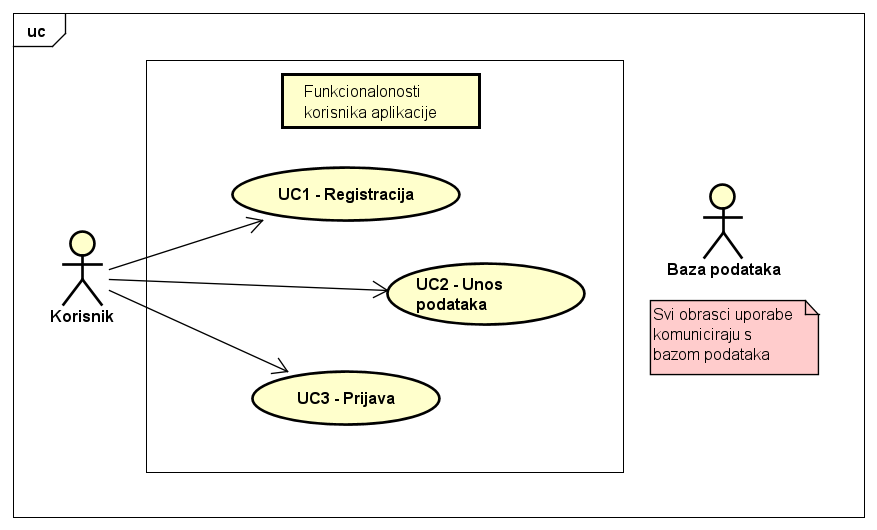
\includegraphics[scale=0.68]{dijagrami/UML_kor.PNG}
						\centering
						\caption{Dijagram obrasca uporabe, funkcionalnost korisnika}
						\label{fig:UML_kor}
					\end{figure}
				\eject
					
					\begin{figure}[h]
						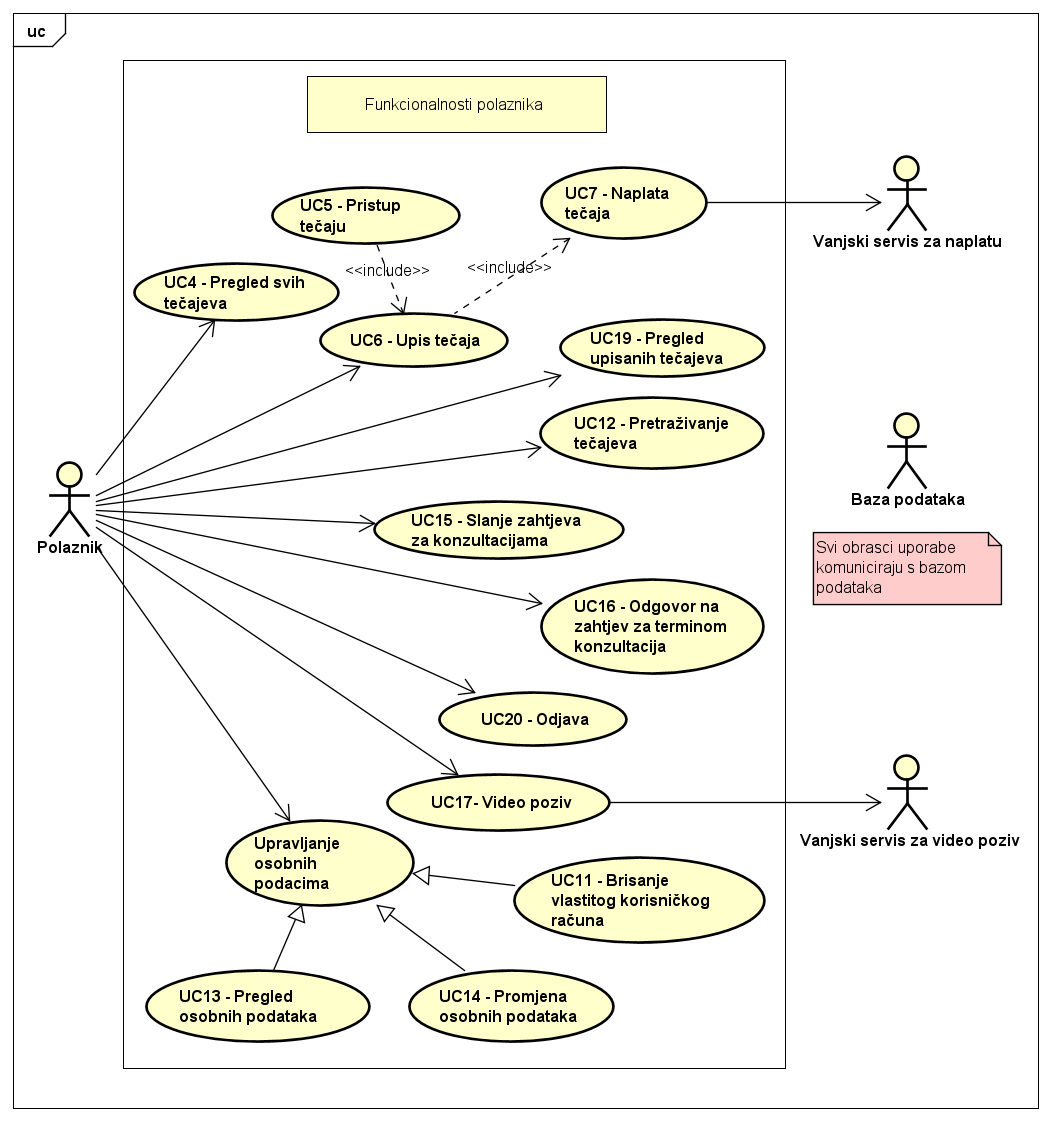
\includegraphics[scale=0.55]{dijagrami/UML_pol.PNG}
						\centering
						\caption{Dijagram obrasca uporabe, funkcionalnost polaznika tečaja}
						\label{fig:UML_pol}
					\end{figure}
				\eject
				
					\begin{figure}[h]
						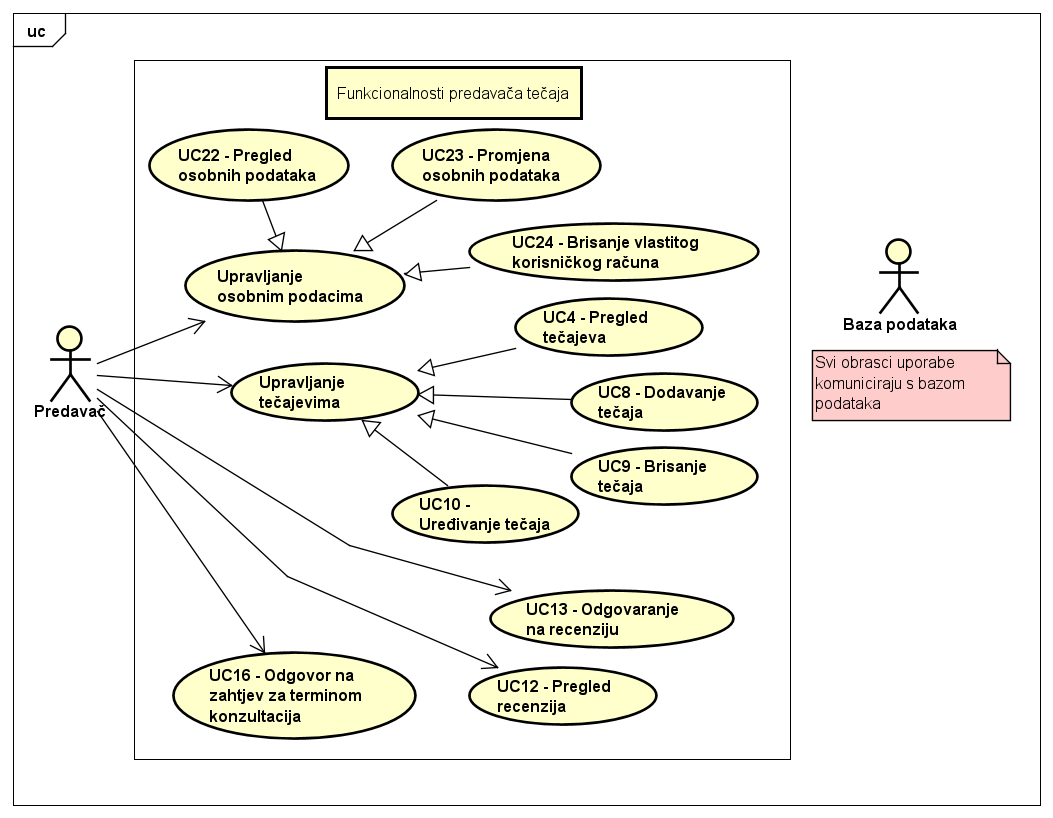
\includegraphics[scale=0.55]{dijagrami/UML_pred.PNG}
						\centering
						\caption{Dijagram obrasca uporabe, funkcionalnost predavača}
						\label{fig:UML_pred}
					\end{figure}
				\eject			
				
			\subsection{Sekvencijski dijagrami}
				
				\subsubsection{Obrasci uporabe UC1 i UC2 - Registracija i Unos podataka}
				
					Korisnik unosi svoju e-mail adresu i željeno korisničko ime. Poslužitelj s bazom podataka provjerava jesu li unesena e-mail adresa i korisničko ime dostupni (nisu zauzeti od strane drugog korisnika). Poslužitelj također provjerava jesu li podaci u dozvoljenom formatu te je li navedena e-mail adresa ispravna. Ako podaci nisu ispravni, sustav korisniku šalje obavijest o neuspjelom upisu i vraća ga na ponovni unos podataka. Ako su podaci ispravni, korisnika se usmjerava na stranicu za unos dodatnih podataka. \newline
					Zatim korisnik unosi dodatne podatke. Ako su potrebni podaci ispravno uneseni, stvara se novi korisnički račun i korisnik dobiva obavijest o uspješnoj registraciji. Ako nije unesen jedan ili više potrebnih podataka, sustav obavještava korisnika. Ukoliko korisnik odluči odustati, registracija se briše.
				\eject
				
					\begin{figure}[h]
						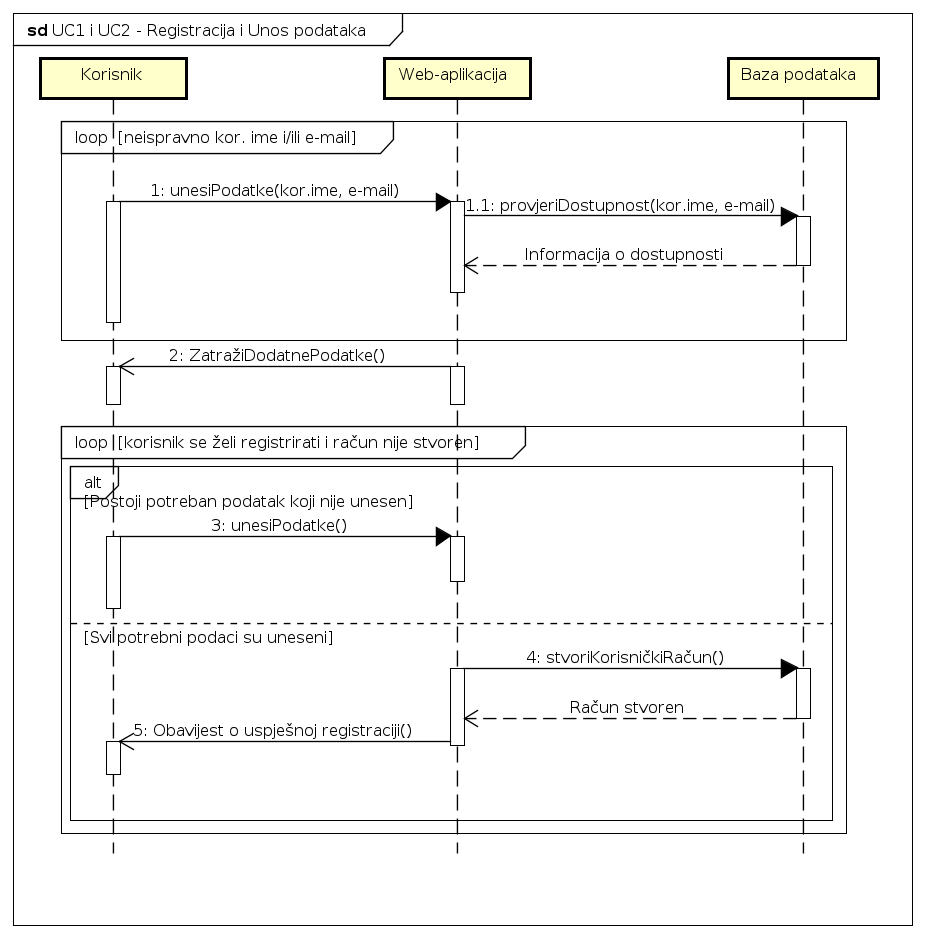
\includegraphics[scale=0.63]{dijagrami/UML_sd_UC1UC2.PNG}
						\centering
						\caption{Sekvencijski dijagram za UC1 i UC2}
						\label{fig:UML_sd_UC1UC2}
					\end{figure}
				
				\eject
				\subsubsection{Obrasci uporabe UC6 i UC7 - Upis tečaja i Naplata tečaja}
				
					Polaznik odabire tečaj koji želi upisati. Nakon odabira tečaja, sustav usmjerava polaznika na stranicu za naplatu. \newline
					Polaznik potvrđuje odabrani tečaj i iznos naplate, a zatim izvršava plaćanje tečaja. Ako na kartici ima dovoljno sredstava, tečaj se plaća i korisnik dobiva pristup tečaju. Ukoliko na kartici nema dovoljno sredstava, sustav obavještava korisnika o nemogućnosti pohađanja tečaja zbog financija.
				
					\begin{figure}[h]
						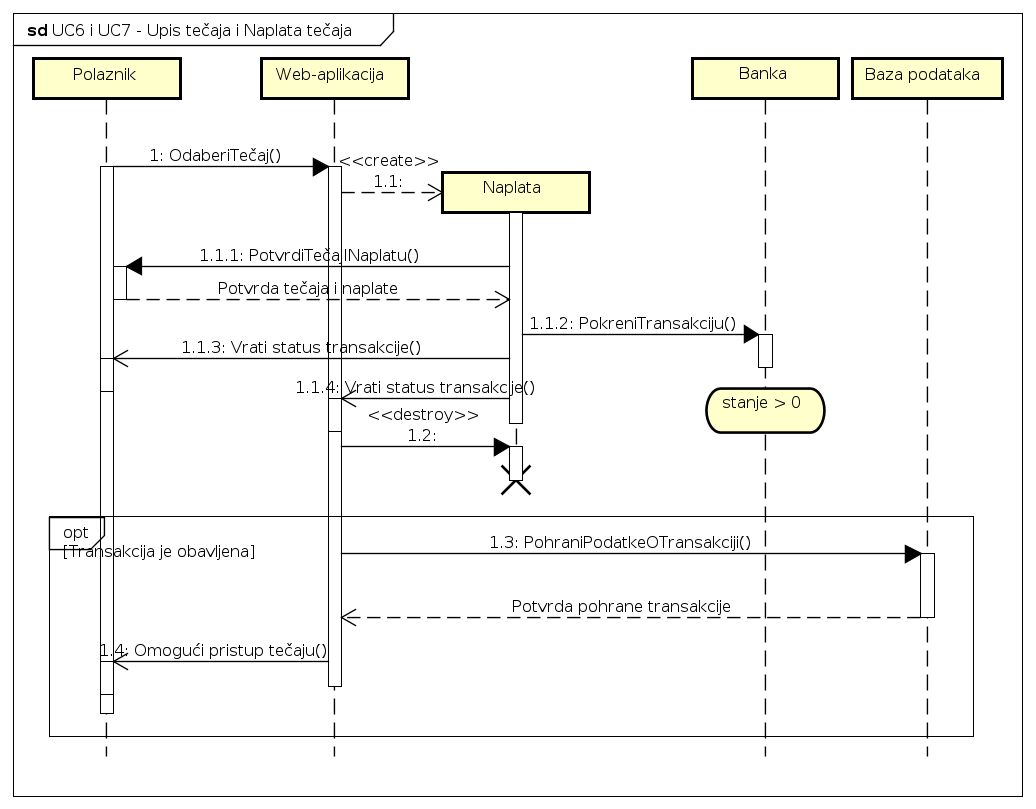
\includegraphics[scale=0.56]{dijagrami/UML_sd_UC6UC7.PNG}
						\centering
						\caption{Sekvencijski dijagram za UC6 i UC7}
						\label{fig:UML_sd_UC6UC7}
					\end{figure}
				
				\eject
				\subsubsection{Obrasci uporabe UC15 i UC16 - Slanje zahtjeva za konzultacijama i Odgovor na zahtjev za terminom konzultacija}
				
					Polaznik šalje zahtjev za terminom konzultacija. Podaci o zahtjevu se pohranjuju u bazu podataka. \newline
					Nakon što je zahtjev pohranjen u bazu podataka, 	poslužitelj predavaču šalje obavijest o dospjelom zahtjevu. Predavač šalje poslužitelju zahtjev za prikaz liste zahtjeva za terminima konzultacija. Poslužitelj dohvaća listu zahtjeva iz baze podataka i prikazuje ih predavaču. Predavač može prihvatiti ili odbiti predloženi termin konzultacija. Ako predavač prihvati termin, poslužitelj izmjenjuje zahtjev u bazi podataka koja vraća potvrdu o odobrenom zahtjevu. Poslužitelj tada šalje obavijest polazniku da je zahtjev odobren. Ako predavač odbije termin, poslužitelj briše poslani zahtjev iz baze podataka i obavještava polaznika da je zahtjev odbijen. Polaznik zatim ponovno šalje zahtjev za terminom konzultacija, sve dok mu se zahtjev ne odobri.
				\eject
				
					\begin{figure}[h]
						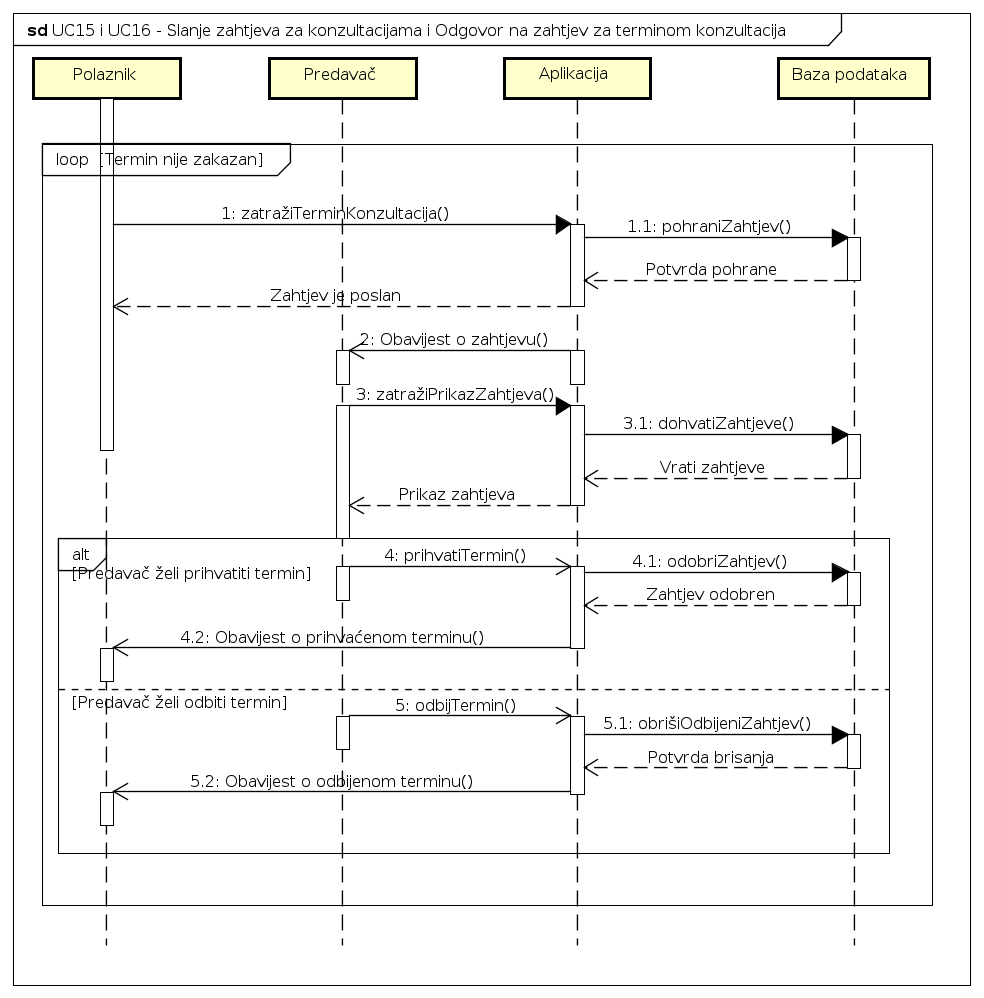
\includegraphics[scale=0.59]{dijagrami/UML_sd_UC15UC16.PNG}
						\centering
						\caption{Sekvencijski dijagram za UC15 i UC16}
						\label{fig:UML_sd_UC15UC16}
					\end{figure}
				\eject
				
		\section{Ostali zahtjevi}
		
			\begin{packed_item}
				\item Sustav treba podržavati rad više korisnika u isto vrijeme
				\item Sustav treba biti jednostavan za korištenje, korisnici se moraju znati koristiti sučeljem bez opširnih uputa
				\item Neispravno korištenje sučelja ne smije narušiti funkcionalnost i rad sustava
				\item Sustav kao valutu koristi HRK
				\item Nadogradnja sustava ne smije narušavati postojeće funkcionalnosti sustava
				\item Korisničko sučelje i sustav moraju podržavati hrvatsku abecedu (dijakritičke znakove) pri unosu i prikazu tekstualnog sadržaja
				\item Veza s bazom podataka mora biti kvalitetno zaštićena, brza i otporna na vanjske greške
				\item Aplikacija mora imati responzivno korisničko sučelje
				\item Svi osobni podaci u aplikaciji moraju se čuvati u skladu s GDPR regulativom
			\end{packed_item}
			 
			 
			 
	